\documentclass[a4paper,12pt]{article}
\usepackage{geometry}
 \geometry{
 a4paper,
 total={170mm,257mm},
 left=20mm,
 top=20mm,
 }
\usepackage{natbib}
%opening

%\usepackage[version=3]{mhchem} % Formula subscripts using \ce{}
\usepackage{braket}
\usepackage{amsmath}
\usepackage{wrapfig}
\usepackage{lipsum}     % for sample text
\usepackage{upgreek}
\usepackage{graphicx}
\usepackage{chemfig}
\usepackage{caption}
\usepackage{textcomp}
\usepackage{underscore}
\usepackage{gensymb}
\usepackage{dcolumn}
\usepackage{siunitx}
\usepackage{multirow}
\usepackage{amssymb}


\begin{document}

\section{Question 1 - Book 4.1}
We will follow the same procedure outlined here for each part of the problem. First, we will calculate $A^*A$ and $AA^*$. From the SVD relationship, we know that $A=U\Sigma V^*$, $A^* =V\Sigma^*U^*$, $AA^* =U\Sigma \Sigma^* U^*$, and $A^*A= V\Sigma^* \Sigma V^*$. So we first take $det(A^*A -\lambda I) =0$ to determine the squared eigenvalues, after which we can build $\Sigma$. Once this is done, we will use these values in $AA^* U=U\Sigma \Sigma^*$ and $A^*A V=V\Sigma^* \Sigma$ to determine $U$ and $V$, using the constraint that both $U$ and $V$ must be unitary. Furthermore, we note that $\Sigma \in \mathbb{C}^{m\times n}$, $U\in \mathbb{C}^{m\times m}$, and $V\in \mathbb{C}^{n\times n}$


\subsection{part a}
det($A^*A - \lambda I$) =0 $\rightarrow \lambda=9,4$

\begin{equation}
\Sigma =\begin{pmatrix}
3&0	\\
0&2\\ 
\end{pmatrix}
\end{equation}



\begin{equation}
AA^*U=\begin{pmatrix}
9&0	\\
0&4\\ 
\end{pmatrix}  U = U\begin{pmatrix}
9&0	\\
0&4\\ 
\end{pmatrix} \rightarrow U=\begin{pmatrix}
1&0	\\
0&1\\ 
\end{pmatrix}
\end{equation}

Instead of calculating $A^*V$ to find $V$, I will instead use the relationship $AV=U\Sigma$ to define $V$, as there is a sign issue if I follow the advice I outlined above. To be honest, it's not immediately clear how I can know - without checking - how to pick the appropriate signs. If I had not multiplied $U\Sigma V^*$ out using advice from above, I would have gotten the wrong answer. 
\begin{equation}
AV=U\Sigma \rightarrow \begin{pmatrix}
3&0	\\
0&-2\\ 
\end{pmatrix} V= 
\begin{pmatrix}
1&0	\\
0&1\\ 
\end{pmatrix} 
\begin{pmatrix}
3&0	\\
0&2\\ 
\end{pmatrix} \rightarrow V= \begin{pmatrix}
1&0	\\
0&-1\\ 
\end{pmatrix}
\end{equation}



\subsection{part b}
det($A^*A - \lambda I$) =0 $\rightarrow (4-\lambda)(9-\lambda)=0 \rightarrow \lambda=4,9$ 
 
\begin{equation}
\Sigma =\begin{pmatrix}
3&0	\\
0&2\\ 
\end{pmatrix}
\end{equation}

\begin{equation}
AA^*U=\begin{pmatrix}
4&0	\\
0&9\\ 
\end{pmatrix}  U = U\begin{pmatrix}
9&0	\\
0&4\\ 
\end{pmatrix} \rightarrow U=\begin{pmatrix}
0&1	\\
1&0\\ 
\end{pmatrix}
\end{equation}

\begin{equation}
A^*AV=\begin{pmatrix}
4&0	\\
0&9\\ 
\end{pmatrix}  V = V\begin{pmatrix}
9&0	\\
0&4\\ 
\end{pmatrix} \rightarrow V=\begin{pmatrix}
0&1	\\
1&0\\ 
\end{pmatrix}
\end{equation}


\subsection{part c}
det($A^*A - \lambda I$) =0 $\rightarrow (4-\lambda) =0 \rightarrow \lambda =4,0$
so
\begin{equation}
\Sigma=\begin{pmatrix}
2&0	\\
0&0\\ 
0&0\\ 
\end{pmatrix}
\end{equation}


\begin{equation}
AA^*U=\begin{pmatrix}
4&0&0	\\
0&0&0\\
0&0&0\\ 
\end{pmatrix}  U =U\begin{pmatrix}
4&0&0	\\
0&0&0\\
0&0&0\\ 
\end{pmatrix}  \rightarrow U=\begin{pmatrix}
1&0&0	\\
0&1&0\\
0&0&1\\ 
\end{pmatrix} 
\end{equation}


\begin{equation}
A^*AV=\begin{pmatrix}
0&0	\\
0&4\\ 
\end{pmatrix}  V = V\begin{pmatrix}
4&0	\\
0&0\\ 
\end{pmatrix} \rightarrow  V=\begin{pmatrix}
0&1	\\
1&0\\ 
\end{pmatrix}  
\end{equation}

\subsection{part d}
det($A^*A - \lambda I$) =0 $\rightarrow \lambda=0,2$ so 
\begin{equation}
\Sigma=\begin{pmatrix}
\sqrt2&0	\\
0&0\\ 
\end{pmatrix}
\end{equation}

\begin{equation}
AA^*U=\begin{pmatrix}
2&0	\\
0&0\
\end{pmatrix}  U =U \begin{pmatrix}
2&0	\\
0&0\
\end{pmatrix} \rightarrow U=\begin{pmatrix}
1&0	\\
0&1\
\end{pmatrix} 
\end{equation}

\begin{equation}
A^*AV=\begin{pmatrix}
1&1	\\
1&1\\ 
\end{pmatrix}  V = V\begin{pmatrix}
2&0	\\
0&0\\ 
\end{pmatrix} \rightarrow  V=\frac{\sqrt2}{2}\begin{pmatrix}
1&-1	\\
1&1\\ 
\end{pmatrix}  
\end{equation}

\subsection{part e}
det($A^*A - \lambda I$) =0 $\rightarrow \lambda=0,4$ so 
\begin{equation}
\Sigma=\begin{pmatrix}
2&0	\\
0&0\\ 
\end{pmatrix}
\end{equation}

\begin{equation}
AA^*U=\begin{pmatrix}
2&2	\\
2&2\
\end{pmatrix}  U =U \begin{pmatrix}
2&0	\\
0&0\
\end{pmatrix} \rightarrow U=\frac{\sqrt2}{2}\begin{pmatrix}
1&-1	\\
1&1\
\end{pmatrix} 
\end{equation}

\begin{equation}
A^*AV=\begin{pmatrix}
2&2	\\
2&2\\ 
\end{pmatrix}  V = V\begin{pmatrix}
2&0	\\
0&0\\ 
\end{pmatrix} \rightarrow  V=\frac{\sqrt2}{2}\begin{pmatrix}
1&-1	\\
1&1\\ 
\end{pmatrix}  
\end{equation}


\section{Question 2 }
I need about 10 terms in the outer product to faintly recognize myself, but maybe a few more beyond that to recognize my son. I attribute this to the fact that my coloring is more diverse and shows smaller variation. My son on the other hand is wearing things that vary in color quickly, therefore needing more terms in the expansion to accurately approximate. I need roughly 25 terms in the expansion to recognize both myself and my son with some degree of clarity, although my aunt and and uncle in the background are still blurry. I think most that the important features of the picture are relative, but I suppose having roughly 35 out of the total 600 terms in the outer product expansion gives enough detail where I can clearly make out me, my son, the boat, the background, and to a lesser extend my aunt and uncle. Figure \ref{fig:boat1} shows an example of the decomposition. It's hard to say what the ideal number of terms would be for an arbitrary photo. But obviously this is a pretty efficient algorithm, and barring a photo with a multitude of colors in close proximity, I would say 5-10\% of terms are needed.
\begin{figure}[h]
  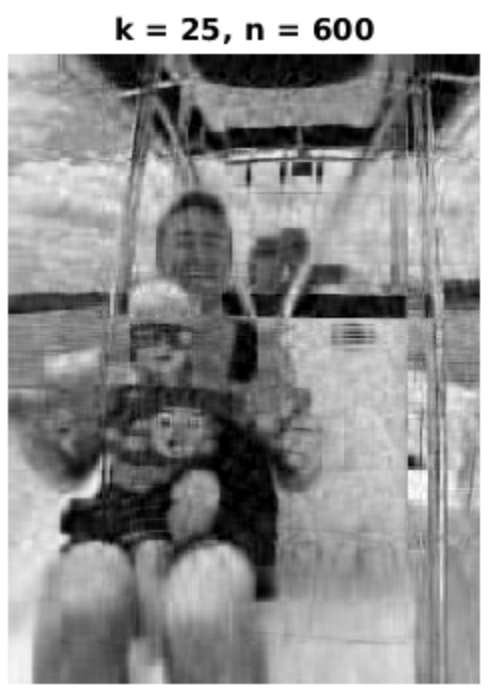
\includegraphics[scale=0.5]{k25.png}
  \caption{SVD with 25 terms in the outer product expansion}
  \label{fig:boat1}
\end{figure}
On a side note: I did not study this code long enough and I am not educated in matlab. But at some point after I learn it in more detail, it would be nice to adopt some of this logic towards developing novel methods for approximating excitations via solution to the Schrodinger equation - which is part of my research. Having understood the highlights of your program, it makes me think that it could be possible to reduce the dimensionality of the matrices we diagonalize to get the excitation energy without significant loss in accuracy. The only problem to this is that I notice you start out by immediately performing the SVD on the entire problem to begin with, then approximate this by adding subsequent terms in the outer product -- so in my case this would offer no time savings if you have to solve the whole problem to begin with. 







\section{Question 3 - Book 6.1}

If $P$ is an orthogonal project, then $P=P^2$ and $P=P^*$ must be satisfied. We want to show that $I-2P$ is unitary. A unitary operator satisfies $UU^*=U^*U=I$. Thus, if we let $U=I-2P$ we see that
\begin{equation}
UU^* = \bigg( I-2P\bigg) \bigg( I-2P\bigg)^*= II^* -2IP^* -2PI^* +4PP^* = I
\end{equation} using the properties of an orthogonal project defined above. Also, we note that

\begin{equation}
U^*U=\bigg( I-2P\bigg)^* \bigg( I-2P\bigg)= I^*I -2I^*P-2P^*I+4P^*P = I
\end{equation} again by using the properties of an orthogonal project defined above. This proves that $I-2P$ is unitary. 



If we have some $v\in range(P)$ such that $Pv=v$, then $(I-2P)v=Iv-2Pv=-v$. As this is a complement to an orthogonal projector, the geometric interpretation is that this operation reflects an arbitrary vector $v$ onto the space orthogonal to $range(P)$, in other words, into the $Nul(P)$.









\section{Question 4 - Book 6.3}
Assuming $A\in \mathbb{R}^{m\times n}$ with $m\geq n$, we will show that $A^*A$ is nonsingular if and only if $A$ has full rank. We begin with the forward proposition, namely that if A has full rank, then $A^*A$ is nonsingular. Consider that if $A$ does not have full rank, there is some $x\neq 0$ such that$Ax=0$. This implies that $A^*Ax=0$ which then implies that $A^*A$ is singular. If this is true, then when $A$ does have full rank, $A^*A$ is nonsingular. 


Now, we will prove the reverse direction. Let $A^*A$ be singular, meaning some $x\neq 0$ such that $A^*Ax=0$. Remembering that $||A||_2=\sigma_1$, we see that $||Ax||_2^2 =x^*(A^*Ax)=0$. This means that the maximum eigenvalue is 0, implying that $A$ cannot be full rank. On the other hand, if $A^*A$ is nonsingular, then $A$ must have full rank. 




\section{Question 5 - Book 6.4}
\subsection{part a}
We can build an orthonormal basis from the columns of $A=(a_1  a_2)$ providing that $a_1 \perp a_2$ and the inner product of the vector with itself is 1. We immediately note the former condition is satisfied. We want to ensure the $(c^* a_1^*)(ca_1) = |c|^2 a_1^*a_1=1$ for some scalar $c$. Performing the dot product, we see that $c=\frac{1}{\sqrt2}$. In addition, we note that $(a_2,a_2)=1$, so $a_2$ is a valuable basis as it is. Thus, the orthonormal basis is $a_1=\frac{1}{\sqrt2}(1,0,1)^*$, $a_2=(0,1,0)^*$. We can then use this knowledge in addition to eq 6.7 to construct the projector.
\begin{equation}
Px=\sum_i^n a_ia_i^* x = \frac{1}{2}\begin{pmatrix}
1\\
0\\
1\\ 
\end{pmatrix}
\begin{pmatrix}
1 & 0&1\\
\end{pmatrix}x +
\begin{pmatrix}
0\\
1\\
0\\ 
\end{pmatrix}
\begin{pmatrix}
0&1&0\\
\end{pmatrix}x
\end{equation} Thus we see that  when $P$ acts on $x^*=(1,2,3)$

\begin{equation}
Px =\begin{pmatrix}
\frac{1}{2}&0&\frac{1}{2}\\
0&1&0\\
\frac{1}{2}&0&\frac{1}{2}\\ 
\end{pmatrix}
\begin{pmatrix}
1\\
2\\
3\\ 
\end{pmatrix} =
\begin{pmatrix}
2\\
2\\
2\\ 
\end{pmatrix}
\end{equation}

\subsection{part b}
Eq 6.13 from the book will be used to define the projection operator, namely $P=B(B^*B)^{-1}B^*$. To begin

\begin{equation}
B^*B=\begin{pmatrix}
2&2\\
2&5\\ 
\end{pmatrix} \rightarrow (B^*B)^{-1} =\frac{1}{10-6}\begin{pmatrix}
5&-2\\
-2&2\\ 
\end{pmatrix}
\end{equation}

So now solving for $P$ gives us
\begin{equation}
P=\frac{1}{6}\begin{pmatrix}
1&2\\
0&1\\
1&0\\ 
\end{pmatrix}
\begin{pmatrix}
5&-2\\
-2&2\\ 
\end{pmatrix}
\begin{pmatrix}
1&0&1\\
2&1&0\\ 
\end{pmatrix} =\frac{1}{6}\begin{pmatrix}
5&2&1\\
2&2&-2\\
1&-2&5\\ 
\end{pmatrix}
\end{equation} When this operator acts on $x^*=(1,2,3)$, the result is
\begin{equation}
Px=\begin{pmatrix}
2\\
0\\
2\\ 
\end{pmatrix}
\end{equation}







\end{document}